
\subsection{Lexical Conventions}

\subsubsection{Assignment}
Every variable in BLAStoff is a matrix.  A matrix variable is defined in the following way:
\begin{lstlisting}
id = expr;
\end{lstlisting}
where the left-hand side is an identifier, which can be made up of alphanumeric characters and underscores, beginning with an alphabetic character, and the right-hand side is an expression.

Matrices can be defined five ways: as a matrix literal, as a graph, as a number, with a generator function, or as a string.  Below we describe are the 5 corresponding expressions.
\paragraph{Matrix Literal Definition}
A matrix literal looks as follows:

\begin{lstlisting}
[row;
 row;
 ...]
\end{lstlisting}
where each \verb=row= looks as follows:
\begin{lstlisting}
num, num, ...
\end{lstlisting}
where each \verb=num= is a positive or negative integer.  Here's an example:
\begin{lstlisting}
M = [1,3,5;
     2,4,6;
     0,0,-1];
\end{lstlisting}
which sets $M$ as the matrix $$\begin{bmatrix}1&3&5\\2&4&6\\0&0&-1\end{bmatrix}$$.

In the matrix literal definition, the number of items ins must be the same in every row.
\paragraph{Graph Definition}
The graph definition looks as follows:
\begin{lstlisting}
[
    (edge | int);
    (edge | int);
    ...
]
\end{lstlisting}
Each \verb=int= is a non-negative integer (\verb=[0-9]+=), and each edge looks as follows:
\begin{lstlisting}
int -> int
\end{lstlisting}
Here's an example:
\begin{lstlisting}
G = {
    0->1;
    1->0;
    1->2;
    4;
};
\end{lstlisting}
This will set $M$ as the adjacency matrix for the graph described, which in this case would be: $$\begin{bmatrix}0&1&0&0&0\\1&0&1&0&0\\0&0&0&0&0\\0&0&0&0&0\\0&0&0&0&0\end{bmatrix}$$  As we can see in this code example, each line in the graph definition can be an edge $a\to b;$ defining a node between vertices $a$ and $b$ where $a,b$ are non-negative integers, or just a vertex $c;$ where $c$ is also a non-negative integer, which just defines that the vertex $c$ exists.  The matrix created will be an $n \times n$ matrix, where $n$ is the highest vertex (in our case 4) defined plus 1.  Thus, the graph created will have nodes $[0,n-1]$.  Any vertices not mentioned in the definition but in the range $[0,n-1]$ will be created, but not have any edges to or from it (such as vertex 3 in this case). \begin{comment}
We could easily extend this syntax to allow for bi-directional or weighted graphs, and will decide later whether to do this.
\end{comment}

\paragraph{Number Definition}
The number definition is quite simple, and looks like as follows:
\begin{lstlisting}
num
\end{lstlisting}
using the
Here's an example:
\begin{lstlisting}
M = 5;
\end{lstlisting}
This is how you would create a  ``scalar'' in BLAStoff, but because the only data type is a matrix, scalars are really $1\times 1$ matrices.  The above code is equivalent to the following code:
\begin{lstlisting}
M = [5];
\end{lstlisting}
which sets $M$ as the matrix $$\begin{bmatrix}5\end{bmatrix}$$
We will discuss in the section on operations how these 1x1 matrices are used to replicate things like scalar multiplication.

\paragraph{Generator Function Definition}
We also have a number of generator functions for commonly-used types of matrices so that you don't waste your time typing out a $50 \times 50$ identity matrix.
This is what they look like:
\begin{lstlisting}
Zero(expr)
I(expr)
range(expr | expr, expr)
\end{lstlisting}

The first is the \verb=Zero= function, which generates a matrix with all 0s.  This takes in one argument, which we will call $x$, a non-negative matrix of two possible sizes.  $n$ can be a $2 \times 1$  positive matrix, and the elements of the $n$ matrix are the height and width of the zero matrix, in that order.  $n$ could also be a $1\times 1$ matrix, in which case the zero matrix will be square, with the element in $n$ as its height and width.  Here is an example:

\begin{lstlisting}
A = Zero(4);
B = Zero([3;2]);
\end{lstlisting}
This code would result in the following matrices:
$$A=\begin{bmatrix}0&0&0&0\\0&0&0&0\\0&0&0&0\\0&0&0&0\end{bmatrix}$$
$$B=\begin{bmatrix}0&0\\0&0\\0&0\end{bmatrix}$$
Note that \verb|A = Zero(4);| is equivalent to \verb|A = Zero([4;4]);|.

We also have an identity function, \verb=I=, which takes in one argument, a $1\times 1$ non-negative matrix, the width and height of the resultant square identity matrix.  Example:\begin{lstlisting}
M = I(3);
\end{lstlisting}
This would result in the following matrix:
$$M=\begin{bmatrix}1&0&0\\0&1&0\\0&0&1\end{bmatrix}$$
The final generator function is the \verb=range= function, which generates a column vector that goes through an integer range, incremented by 1.  Like \verb=Zero=, it takes in an matrix of size $1\times 1$ or size $2\times 1$, which gives the bounds of the range generated (inclusive lower, exclusive upper), or, in the $1\times 1$ case, the exclusive upper bound, and 0 is the default lower bound.  Here are some examples:
\begin{lstlisting}
A = range(3);
B = range(-2,2);
\end{lstlisting}
This code would result in the following matrices:
$$A = \begin{bmatrix}0 \\ 1 \\ 2 \end{bmatrix}$$
$$B = \begin{bmatrix}-2 \\ -1 \\ 0 \\ 1 \end{bmatrix}$$
If a range where the lower bound is greater than the upper bound given to \verb=range=, such as \verb=range([5;-1])=, a $0 \times 1$ matrix will be returned.

\paragraph{String Definition}
The final definiton method is as a string.  It looks like the following:
\begin{lstlisting}
`str`
\end{lstlisting}
where the \verb=str= is any string sequence.  This returns a column vector with the ASCII values of the given string.  For instance;
\begin{lstlisting}
A = `BLAS`
\end{lstlisting}
This code would result in the following matrix:
$$A = \begin{bmatrix}66 \\ 76 \\ 65 \\ 83\end{bmatrix}$$
It will be apparent later how this is useful.

\subsubsection{Comments}
There are two types of comments in BLASToff.  Single-line comments are denoted by \verb=//=.  Multi-line comments begin with  \verb=/*= and end with \verb=*/=.  For example:
\begin{lstlisting}
A = 6; // I'm a comment!
B = 5; /* I'm a comment also but
...
...
I'm longer!*/
\end{lstlisting}

\subsubsection{Functions}
Functions in BLAStoff are defined as follows:\begin{lstlisting}
def id(id, id, ...) {
    stmnt;
    stmnt;
    ...
}
\end{lstlisting}
In functions, returning is optional.  Here is a simple example.
\begin{lstlisting}
def foo(A, B) {
    return A;
}
\end{lstlisting}
Because there is only one data type in BLAStoff, there is no need for argument types or return types, everything is always a matrix!  Even ``void'' functions return matrices.  Consider these two functions:

\begin{lstlisting}
def bar1(A) {
    return;
}

def bar2(A) {
    ;
}
\end{lstlisting}
These two functions both return the equivalent of ``None'' in BLAStoff, a $0\times 0$ matrix.

\subsubsection{If statements}
If/else statements, look as follows:
\begin{lstlisting}
if (expr) stmnt ?[else stmnt]
\end{lstlisting}

For example:
\begin{lstlisting}
if (A > 2) {
    A = 7;
} else if (A < -3) {
    A = 5;
} else {
    A = 0;
}
\end{lstlisting}

The truth value of an \verb=expr= is equivalent to \verb=expr > 0=.  The \verb=>= operator will be discussed in full later.

\subsubsection{For/While Loops}
For and while loops look as follows:
\begin{lstlisting}
for (?expr ; expr ; ?expr) stmnt
while (expr) stmnt
\end{lstlisting}

For example:

\begin{lstlisting}
B = 0;
for (A = [0]; A < 5 ; A+=1) {
    B+=1;
}

while (B > -1) {
    B-=1;
}
\end{lstlisting}
Though we allow for loops, but they are not usually the ideal paradigm.  The selection operator, defined later,  should hopefully replace much of the use for loops.

\subsubsection{Operations}
Operations are where BLAStoff gets more interesting.

We aim to implement a large subset of the basic primitives described in \cite{Gilbert} (several of which can be combined) as well as a few essential semirings.\\\\
\label{sec:semirings}
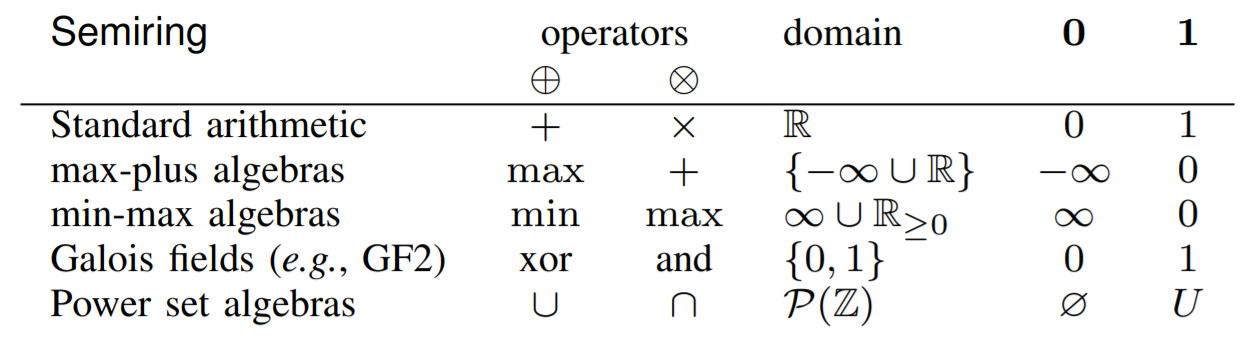
\includegraphics[scale=0.3]{figures/common Semirings.png}\\Do we
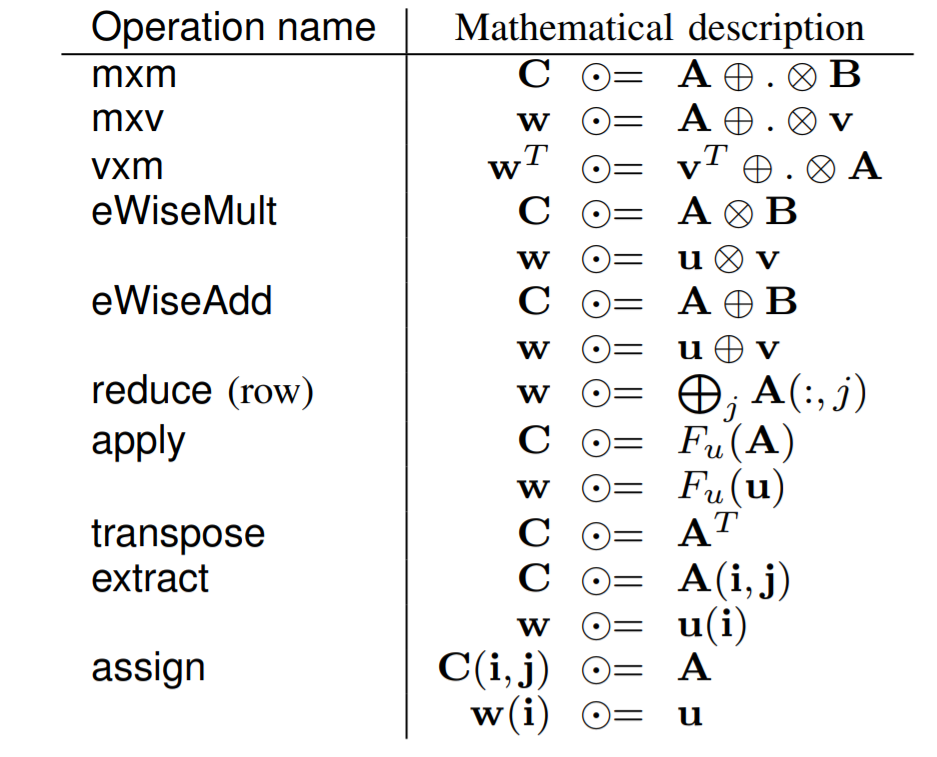
\includegraphics[scale=0.3]{figures/BLAS primitives.png}\\

This is how we implement these operators and some more:

\paragraph{Selection}
Here is the grammar for the selection operator:\begin{lstlisting}
expr[expr, expr, expr, expr];
expr[expr, expr]
expr[expr];
\end{lstlisting}
The BLAStoff selection operator can be applied to any matrix and looks like one of the following three forms:
\begin{lstlisting}
M[A, B, c, d];
M[A, B]
M[A];
\end{lstlisting}
where $A,B$ are column vectors of non-negative integers ($n\times 1$ matrices) and $c,d$ are $1 \times 1$ non-negative matrices.  $c,d$ are optional and have a default value of $\begin{bmatrix}1\end{bmatrix}$. $B$ is also optional and its default value is $\begin{bmatrix}0\end{bmatrix}$.  Abstractly, the way this operator works is by taking the Cartesian product of $A,B$, $R=A\times B$, and for each $(j,i)\in R$, we select all the sub-matrices in $M$ with a top-left corner at row $j$, column $i$, height of $c$, and width of $d$.  (BLAStoff is 0-indexed.)  This Cartesian makes the select operator a very powerful operator that can do things like change a specific of indices, while also being general enough to allow for simple indexing.  Take the following code example:
\begin{lstlisting}
M = Zero(4)
M[[0;2], [0;2]] = 1;
\end{lstlisting}

This would result in the following matrix:
$$M = \begin{bmatrix}
1 & 0 & 1 & 0\\
0 & 0 & 0 & 0\\
1 & 0 & 1 & 0\\
0 & 0 & 0 & 0
\end{bmatrix}$$
as in this case $R=\{(0,0), (0,1), (1,0), (1,1)\}$, so for every $1\times 1$ matrix at each point in $R$, we set the value to 1.  Note that the matrix on the right hand side must be of size $c\times d$.  That was a relatively complicated use of the select operator, but simple uses still have very easy syntax:
\begin{lstlisting}
M = Zero(2);
M[1, 0] = 1;
N = Zero(3);
N[1, 1, 2, 2] = I(2);
\end{lstlisting}
This would result in:
$$M=\begin{bmatrix}0 & 0 \\ 1 & 0\end{bmatrix}$$
$$N=\begin{bmatrix}
0 & 0 & 0\\
0 & 1 & 0\\
0 & 0 & 1\end{bmatrix}$$
The reason why 0 is the default value of $B$ is to allow for easy column vector access.  Example:
\begin{lstlisting}
v = [1;1;1];
v[1] = 2;
u = [1;1;1];
u[[0;2]] = 2;
\end{lstlisting}
This would result in:
$$v=\begin{bmatrix}1\\2\\1\end{bmatrix}$$
$$u=\begin{bmatrix}2\\1\\1\end{bmatrix}$$
Now, perhaps it is clear why we included the \verb=range= generator function.  Example:
\begin{lstlisting}
v = Zero([5;1]);
v[range(5)] = 1;
\end{lstlisting}
This would result in:
$$v=\begin{bmatrix}1\\1\\1\\1\\1\end{bmatrix}$$
As you'd expect, trying to access anything out-of-bounds with the selection operator will throw an error.

We have shown the selection operator so far as a way of setting elements in a matrix, but it's also a way of extracting values from a matrix, as we will show below:
\begin{lstlisting}
A = [1,2,3;
    4,5,6;
    7,8,9];
B = A[0, 0, 2, 2];
\end{lstlisting}
This would result in:
$$B=\begin{bmatrix}1 & 2\\4 &5 \end{bmatrix}$$
Extraction is quite understandable when $A$ and $B$ are $1\times 1$, as that results in only one matrix, but it is a bit more complicated when they are column vectors.  In that case, we concatenate the number of resultant matrices, both vertically and horizontally.  I think an example makes this clearer:
\begin{lstlisting}
A = [1,2,3;
    4,5,6;
    7,8,9];
B = A[[0;2], [0;2] , 1, 1];
v = [1;2;3;4];
u = v[[0;2;3]];
\end{lstlisting}
This would result in:
$$B=\begin{bmatrix}1 & 3\\7 &9 \end{bmatrix}$$
$$u=\begin{bmatrix}1\\3\\4\end{bmatrix}$$

\begin{comment}
Do something about intersecting selections
\end{comment}

\paragraph{Matrix Multiplication}
We now define a number of binary operators.  The grammars for these operators all look like
\begin{lstlisting}
expr % expr
\end{lstlisting}
where \verb=%= is the given operator.

The matrix multiplication operator \verb=*= looks like the following:
\begin{lstlisting}
A*B
\end{lstlisting}
where $A$ is an $l\times m$ matrix and $B$ is an $m \times n$ matrix.  The product is an $l \times n$ matrix.  This operation works like standard matrix multiplication, so I don't have to spend 2 pages explaining how it works, like I did for selection.  Here's an example:
\begin{lstlisting}
A = [1,2;
    1,2;
    1,2;
    1,2]
B = [1,2,3;
    1,2,3;]
C = A*B;
\end{lstlisting}
This would result in:
$$C=\begin{bmatrix}3 & 6 & 9\\3 & 6 & 9\\3 & 6 & 9\\3 & 6 & 9\end{bmatrix}$$

\paragraph{Convolution}
The convolution operator \verb=~= looks like the following:
\begin{lstlisting}
A~B
\end{lstlisting}
where $A$ is an $m\times n $ matrix and $B$ is an $o\times p$ matrix such that $m\geq o$, $n\geq p$, and $o,p>0$.  The output is an $(m-o+1)\times (n-p+1)$ matrix.  It works like normal matrix convolution, where $B$ is the kernel and the output of $A.B$ is the result of sliding the kernel, $B$, along each row of the matrix $A$ and taking the sum of the element-wise product of the kernel and the sub-matrix it covers. Here is an example:
\begin{lstlisting}
A = [1,2,3;
    4,5,6;
    7,8,9];
B = I(2);
C = A~B;
\end{lstlisting}
This would result in:
$$C=\begin{bmatrix}
6&8\\
12&14
\end{bmatrix}$$
The convolution operator can be used to achieve some other typical operators in Linear Algebra.  For instance, scalar multiplication:
\begin{lstlisting}
k = 2;
A = [1,2,3;
    4,5,6;
    7,8,9];
B = A~k;
\end{lstlisting}
This would result in:
$$B=\begin{bmatrix}
2&4&6\\
8&10&12\\
14&16&18
\end{bmatrix}$$
Or the dot product:
\begin{lstlisting}
v1 = [1;2];
v2 = [2;3];
u = v1~v2;
\end{lstlisting}
This would result in:
$$u=\begin{bmatrix}
8
\end{bmatrix}$$

\paragraph{Element-wise Multiplication}
The element-wise multiplication operator \verb=@= looks like the following:
\begin{lstlisting}
A@B
\end{lstlisting}
where $A$ and $B$ are both $m\times n$ matrices.  The output is also a $m \times n$ matrix. This is standard element-wise multiplication, and is rather straightforward.  Example:
\begin{lstlisting}
A = [1,2;
    3,4];
B = [5,6;
    7,8];
C = A@B;
\end{lstlisting}
This would result in:
$$C=\begin{bmatrix}
5&12\\
21&32\\
\end{bmatrix}$$

\paragraph{Element-wise Addition}
The element-wise addition operator \verb=@= looks like the following:
\begin{lstlisting}
A+B
\end{lstlisting}
where $A$ and $B$ are both $m\times n$ matrices.  The output is also a $m \times n$ matrix. This is standard element-wise addition/matrix addition, and is also rather straightforward.  Example:
\begin{lstlisting}
A = [1,2;
    3,4];
B = [5,6;
    7,8];
C = A+B;
\end{lstlisting}
This would result in:
$$C=\begin{bmatrix}
6&8\\
10&12\\
\end{bmatrix}$$

\cprotect\paragraph{Exponentiation}
The exponentiation operator \verb=^= looks like one of the following forms:
\begin{lstlisting}
expr^(expr | T)
\end{lstlisting}
We can say these correspond to
\begin{lstlisting}
A^b
A^T
\end{lstlisting}
First we will look at the $A^b$ case.  In this case, $A$ is an $n\times n$ (square) matrix and $b$ is a $1\times 1$ positive matrix.  The output will be an $n\times n$ matrix as well.  This operator is normal matrix exponentiation.  For example:
\begin{lstlisting}
A = [1,2;
    3,4];
B = A^2;
\end{lstlisting}
This would result in:
$$B=\begin{bmatrix}
6&8\\
10&12\\
\end{bmatrix}$$

In the $A^T$ case, $A$ is any $m\times n$ matrix, and $T$ is a reserved keyword.  This returns the transpose of $A$, an $n \times m$ matrix.  Example:
\begin{lstlisting}
A = [1,2,3;
    4,5,6];
B = A^T;
\end{lstlisting}
This would result in:
$$B=\begin{bmatrix}
1&4\\
2&5\\
3&6
\end{bmatrix}$$

\paragraph{Size}
The size operator \verb=||=  looks like the following:
\begin{lstlisting}
|expr|
\end{lstlisting}
where the value of the expression, $A$, is any $m\times n$ matrix and returns the $2\times 1$ matrix/column vector
$$\begin{bmatrix}m\\n\end{bmatrix}$$
Example:
\begin{lstlisting}
A = [1,2,3;
    4,5,6];
B = |A|;
\end{lstlisting}
This would result in:
$$B=\begin{bmatrix}
2\\3
\end{bmatrix}$$
Note that this format is the same as the argument to \verb=Zero=!  So, consider the following code:
\begin{lstlisting}
C = Zero(|A|);
\end{lstlisting}
This would result in $C$ being a matrix of the same size as $A$, but all zeroes!  How convenient!

Of course, if you want to extract the number of rows and columns individually, you can use our selection operator:
\begin{lstlisting}
m = |A|[0];
n = |A|[1];
\end{lstlisting}
Combining this with another selection operator and the \verb=range= function, we can do things like replace every element in $A$ with an arbitrary number, not just 0:
\begin{lstlisting}
A[range(m), range(n)] = 5;
\end{lstlisting}

\paragraph{Vertical Concatenation}
The vertical concatenation operator \verb=:= is another binary operator, and looks like one the following:
\begin{lstlisting}
A:B
\end{lstlisting}
where $A$ is an $m \times n$ matrix and $B$ is an $l \times n$ matrix.  The output will be an $(m+l) \times n $ matrix, that consists of $A$ on top of $B$.  Example:
\begin{lstlisting}
A = [1,2];
B = [3,4;
    5,6];
C = A:B;
\end{lstlisting}
This would result in:
$$C=\begin{bmatrix}
1&2\\
3&4\\
5&6
\end{bmatrix}$$

\paragraph{A note on horizontal concatenation}
\label{sec:2.6.8.1}
We do not have horizontal concatenation operator.  Why is this?  Do we hate the horizontal direction?  No, it is because you can easily write an efficient function for horizontal concatenation using vertical concatenation, and we will show that function below.  In general, any potential operator that can be written as a function, but doesn't employ for loops heavily, that is just as effective as implementing a primitive, we do not use an operator for, and instead put it in our standard library, discussed below.

(It is also worth noting that you can construct an efficient function for vertical concatenation using horizontal concatenation, but we have to choose one of them, and vertical is preferable as BLAStoff uses column vectors more often than row vectors).


\paragraph{Reduce Rows}
The reduce rows operator \verb=%=,  looks like the following:
\begin{lstlisting}
(+|*)%expr
\end{lstlisting}
So, the two possible forms are
\begin{lstlisting}
+%A
*%A
\end{lstlisting}
Here, if $A$ is an $m\times n$ matrix, this will output an $m \times 1$ matrix, a column vector.

If $$A=\begin{bmatrix}
A_{0,0} & A_{0,1} & \dots & A_{0,n-1}\\
A_{1,0} & A_{1,1} & \dots & A_{1,n-1}\\
\vdots&\vdots&\vdots&\vdots\\
A_{m-1,0} & A_{m-1,1} & \dots & A_{m-1,n-1}\\
\end{bmatrix}$$
then
$$+\$A=\begin{bmatrix}
\sum_{i=0}^{n-1} A_{0, i}\\
\sum_{i=0}^{n-1} A_{1, i}\\
\vdots\\
\sum_{i=0}^{n-1} A_{m-1, i}\\
\end{bmatrix}$$
and
$$*\$A=\begin{bmatrix}
\prod_{i=0}^{n-1} A_{0, i}\\
\prod_{i=0}^{n-1} A_{1, i}\\
\vdots\\
\prod_{i=0}^{n-1} A_{m-1, i}\\
\end{bmatrix}$$
Here's a code example:
\begin{lstlisting}
A = [1,2;
    3,4;
    5,6];
B = +%A;
C = *%A;
\end{lstlisting}
This would result in:
$$B=\begin{bmatrix}
3\\
7\\
11\\
\end{bmatrix}$$
$$C=\begin{bmatrix}
2\\
12\\
30\\
\end{bmatrix}$$

\paragraph{A note on reduce columns}
See \hyperref[sec:2.6.8.1]{2.6.8.1}.

\paragraph{Assignment operators}
The operator \verb|*=|, used as follows:
\begin{lstlisting}
A*=B;
\end{lstlisting}
is equivalent to
\begin{lstlisting}
A = A*B;
\end{lstlisting}
The same is true for the other assignment operators:
\begin{lstlisting}
A~=B;
A@=B;
A+=B;
A^=b;
A:=B;
\end{lstlisting}


\paragraph{Comparisons}

The comparison operators, all typical binary operators,  can be used as follows:\begin{lstlisting}
A == B
A != B
A > B
A >= B
A < b
A <= B
\end{lstlisting}
where $A$ and $B$ are both $m\times n$ matrices.  These operations return our version of ``true,'' $\begin{bmatrix}1\end{bmatrix}$ if these comparisons are hold element-wise in $A$ and $B$.  That, is $\forall (j,i) \in ([0,m) \times [0, n))$, $A_{j,i} \geq B_{j,i}$, using the \verb|>=| operator as an example.  Note that $>$ and $<$ are not anti-symmetric under this definition.
The one exception to the element-wise rule is $\verb|!=|$, which is just logical not on \verb|==|.

\paragraph{Semiring redefinition}
You may have noticed that though we have defined a number of operations on matrices, when we are actually computing these matrix operations, in our examples the only operators we have actually used on the elements of these matrices are have been standard arithmetic $+$ and $\times$.  However, we want to be able to use a number of semiring operators, such as those defined in \hyperref[sec:semirings]{the image above}.  BLAStoff allows for semiring redefinition in one of the following forms:
\begin{lstlisting}
#logical
#arithmetic
#maxmin
#_
\end{lstlisting}
So what does this syntax actually do?  Ignore the underscore case for now.  The other three are commands to switch the command to the one denoted in the brackets.  Let's see an example:

\begin{lstlisting}
a = 2.1;
b = 3;
c = 0;

#arithmetic;
a + b; //returns 5.1
a * b; //returns 6.3
a * c; //returns 0

#logical;
a + b; //returns 1: plus is now logical or; 0 is the only false value and 1 is the default true value
a * b; //returns 1 as well: times is now logical and
a * c; //returns 0


#maxmin;
a + b; //returns 2.1; plus is now minimum
a * b; //returns 3; times is now maximum
a * c; //returns 2.1
\end{lstlisting}

\verb=#arithmetic= is the default, so that line was technically redundant, but included for clarity.
The example we gave was with $1\times1$ matrices, but the semiring definitions work on matrices of any size:

\begin{lstlisting}
A = [1,4;
    6,3];
B = [5,2;
    7,1];
C = A + B;
\end{lstlisting}
This would result in:
$$C=\begin{bmatrix}
1&2\\
6&1
\end{bmatrix}$$
Semiring redefinition generally is reset back to the default arithmetic when you call a function:
\begin{lstlisting}
def add(x, y) {
    return x + y;
}

a = 4;
b = 3;
#logical;

a + b; // will return 1
add(a, b); // will return 7
\end{lstlisting}
But we provide the \verb=#_= in order to solve this: calling that command will set the semiring to whatever it was as this function was called (or to arithmetic as a default if you're not in a function):
\begin{lstlisting}
def semiringAdd(x, y) {
    #_;
    return x + y;
}

a = 4;
b = 3;
#logical;

a + b; // will return 1
semiringAdd(a, b); // will also return 1
\end{lstlisting}

\paragraph{Logical Negation}
The final operator is logical negation \verb=!=.  It looks as follows:
\begin{lstlisting}
!expr
\end{lstlisting}
where the value of the \verb=expr=, $A$, is any $m \times n$ matrix.  It outputs an $m \times n$ matrix where each element is logically negated.  That is, all zeroes become ones and all non-zeroes become zeroes.  Here is an example:

\begin{lstlisting}
A = [1,0;
    0,3];
B = !A;
\end{lstlisting}
This would result in:
$$B=\begin{bmatrix}
0 & 1\\
1 & 1
\end{bmatrix}$$
This operator's behavior is invariant of the semiring, as do selection, transpose, inverse, vertical concatenation, and size.

\subsubsection{Precedence}
Below is the precedence table for operators, from highest to lowest:
\begin{center}
\begin{tabular}{|c|c|c|}
    \hline
    Operator &  Symbol & Associativity\\
    \hline
    Exponentiation & \verb|^| & Right\\
    \hline
    Selection & \verb|[]| & Left\\
    \hline
    Logical Negation & \verb|!| & Right\\
    \hline
    Reduce Rows & \verb|+%|, \verb|*%| & Right\\
    \hline
    Vertical Concatenation & \verb|:| & Left\\
    \hline
    Multiplications/Convolution &  \verb|*|, \verb|~|, \verb|@| & Left\\
    \hline
    Addition &  \verb|+| & Left\\
    \hline
    Comparisons &  \verb|<|, \verb|>|, \verb|==|, \verb|<=|, \verb|>=|  & Left\\
    \hline
\end{tabular}
\end{center}

\subsubsection{Keywords}
BLAStoff reserves the following keywords:
\begin{verbatim}
I, Zero, range, def, return, if, else, for, while, T, print, inf
\end{verbatim}

\subsection{More Language Details}
\subsubsection{Memory}
BLAStoff will use pass-by-reference, return-by-reference and assign-by-value.  Here's an example of how this will works:
\begin{lstlisting}
def f(x){
    x += 1;
}
a = 1;
f(a);
a == 1; //FALSE
a == 2; //TRUE

b = 1;
c = b;
c += 1;
c == 2; //TRUE
b == 2; //FALSE
b == 1; //TRUE
\end{lstlisting}

Because we use assign-by-value, each matrix has a reference count of 1, and garbage collection is quite simple; you simply de-allocate all variables declared in a function after the function ends.

\subsubsection{Scope}
BLAStoff has scope shared between blocks in the same function call, but not in different function calls.   Example:
\begin{lstlisting}

a = 1;
{
    b = 2 + a; // valid
}
c = b + 1; // valid

def f(x){
    return x * (b + c); // error
}
\end{lstlisting}

\subsubsection{Printing}
We provide the primitive function \verb=print= that takes in one non-negative column vector, with all values less than 127, and prints the corresponding ASCII characters.  As you may suspect, this is a good use of the string matrix definition:
\begin{lstlisting}
print("Hello World!\n");

OUTPUT:
Hello World!
\end{lstlisting}
We also provide a standard library function \verb=toString= that takes in any matrix and returns a column vector corresponding to the pretty-printed string:
\begin{lstlisting}
A = [1, 2;
    3, 4];
print(toString(A));

OUTPUT:
1 2
3 4
\end{lstlisting}

\subsection{Sample Code}

\subsubsection{Some Standard Library Functions}
As we have discussed, we intend to provide a standard library that should have include a good number of the other linear algebra operations that aren't primitives.  Here are some examples:

\paragraph{One}
\verb=One= works exactly like \verb=Zero=, but has all 1s in the matrix:
\begin{lstlisting}
def One(size){
    A = Zero(size);
    m = size[0];
    A[range(size[0]), range(size[1])] = 1;
    return A;
}
\end{lstlisting}

\paragraph{Horizontal Concatenation}
As we said, we don't include this as an operator because it is quite easy to write as a function using vertical concatentation and transpose:
\begin{lstlisting}
def horizontalConcat(A, B){
    return (A^T:B^T)^T;
}
\end{lstlisting}

\paragraph{Plus/Times Column Reduce}
Column reduction follows similarly:
\begin{lstlisting}
def plusColumnReduce(A){
    #_;
    return ((+%A)^T)^T;
}

def timesColumnReduce(A){
    #_;
    return ((*%A)^T)^T;
}
\end{lstlisting}

\paragraph{Sum}
\verb=sum= gives you the sum of all the elements in the matrix.  There are two simple $O(N)$ implementations (where $N$ is the total number of elements in the matrix), and I'll provide both options as an example:
\begin{lstlisting}
def sum(A){
    #_;
    return A~One(|A|);
}

def sum(A){
    #_;
    return plusColumnReduce(+%A);
}
\end{lstlisting}

\paragraph{Range From Vector}
\verb=rangeFromVector= takes in a column vector and returns a vector of the indices that have non-zero.  For instance:
$$\text{rangeFromVector}(\begin{bmatrix}
0 \\ 1 \\ 1 \\ 0 \\ 1
\end{bmatrix})
=
\begin{bmatrix}
1\\2\\4
\end{bmatrix}
$$
This will come in handy in the BFS algorithm that we will write:
\begin{lstlisting}
def rangeFromVector(v){
    #logical;
    vlogic = v~1;
    #arithmetic;
    n = plusColumnReduce(v); // the number of non-zero values
    u = Zero(n, 1);
    j = 0;
    for (i = 0; i < |v|[0]; i += 1) {
        if (v[i]) {
            u[j] = i;
            j++;
        }
    }
}
\end{lstlisting}



\subsubsection{Graph Algorithms}
Here we demonstrate how pseudocode from a 2019 presentation by John Gilbert describing BFS in linear algebraic terms \cite{Gilbert} can be expressed in BLAStoff\\
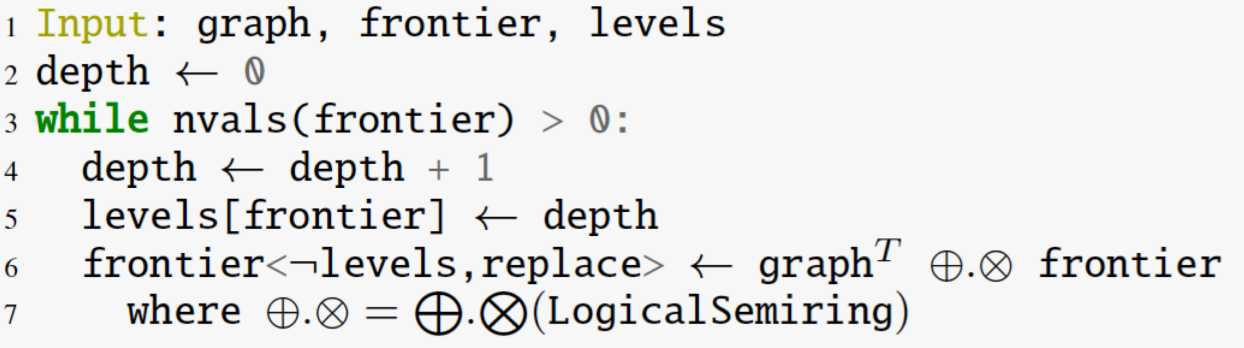
\includegraphics[scale=0.4]{figures/graphBLAS BFS pseudocode.png}\\
Our code for BFS looks like the following:
\begin{lstlisting}
def BFS(G, frontier){
    #logical;
    N = |G|[0];
    levels = Zero(N, 1);
    maskedGT = G^T;
    depth = 0;
    while (sum(frontier)) {
        #arithmetic;
        depth += 1;
        #logical;
        levels[rangeFromVector(frontier)] = depth;
        mask = !(frontier^T)[Zero(N), 0, 1, N];
        maskedGT @= mask;
        frontier = maskedGT*frontier;
    }
    #arithmetic;
    return levels + (One(|levels|~(-1));
}
\end{lstlisting}
Let's look at how this code works.  It takes in an $n\times n$ adjacency matrix $G$ and a column vector $frontier$ of height $n$ as well, where each entry is 0 or a true value, to denote whether that vertex is in the starting list.  On line 4, we then create $levels$, a vector of the same size as $frontier$.  This will be our output vector, as it $levels[i]$ will contain the closest distance from vertex $i$ to a vertex in frontiers, or $-1$ if its unreachable.   You'll notice that we initialize $levels$ with 0s as we will decrement on line 17.  We then make a new variable $maskedGT$ on line 5, which is just the transpose of $G$.  We do this because we are going to be modifying this matrix, but we don't want to change the original $G$.  We take the transpose because that's what allows for part of the algorithm, which I'll explain in a second, and we don't want to do that on every iteration. We then set a variable $depth$ to 0 on 6.  This will keep track of our iterations.

Then we start the while loop, which keeps going as long as there is one non-zero value in $frontier$; that is, we still have vertices we want to look at.  We then increment depth on line 9, switching quickly to arithmetic for this one line, as otherwise depth would never go above 1.  Using our range-from-vector function defined in the standard library, line 11 essentially sets $levels[i]$ equal to the current depth if $frontier[i]$ is non-zero.  That way, all the vertices that we're currently searching for have their distance in levels as the current iteration in our while loop.  This will be one more than the level, but we're going to decrement on line 17.   The key portion of this code is line 14, which mutilates $maskedGT\cdot frontier$.  Because of the way the adjacency matrix is constructed, this will give us a vector in the same format as $frontier$, only now with the vertices reachable from the vertices in the original $frontier$, and we will overwrite $frontier$ with this new frontier.  With all that I've explained so far, the algorithm would be give you the correct reachable nodes, but would run over paths to vertices for which we've already found a closer path, so depths would be wrong.

To account for this, on lines 12 and 13 we remove all the edges to the nodes in frontier, so that as we continue in BFS, we add a previously visited node.  We generate a mask by taking our frontier, transposing it, concatenating it down $N$ times, and negating it.  Here's an example:
$$frontier = \begin{bmatrix}0 \\1\\1\\0\\0\\1\end{bmatrix}$$
$$\begin{bmatrix}0&1&1&0&0&1\end{bmatrix}$$
$$\begin{bmatrix}
0&1&1&0&0&1\\
0&1&1&0&0&1\\
0&1&1&0&0&1\\
0&1&1&0&0&1\\
0&1&1&0&0&1\\
0&1&1&0&0&1
\end{bmatrix}$$
$$\begin{bmatrix}
1&0&0&1&1&0\\
1&0&0&1&1&0\\
1&0&0&1&1&0\\
1&0&0&1&1&0\\
1&0&0&1&1&0\\
1&0&0&1&1&0
\end{bmatrix}$$
In this map, all the ones denote edges not to items in frontier, and thus edges we can keep.  So, if we do element-wise multiplication between this mask matrix and our ongoing, masked, $G^T$, we will keep removing those edges and ensure we never revisit!
